%%
%% Author: dariochinelli
%% 2021-04-06
%%


\section{Calore specifico di un solido cristallino}
È stato un problema della fisica affrontato da molti studiosi, come Einstein e Debye, nel corso dei primi del '900, che ha aperto una nuova visione su vari ambiti.
il calore specifico molare a volume costante è definito come
\begin{equation}
c_V = \frac{1}{N} \frac{dU}{dT}
\end{equation}
dove $N$ rappresenta il numero di moli.
Questa grandezza misura l'energia necessaria per far variare di un grado la temperatura di una mole di sostanza.
Un cristallo è una struttura geometrica in cui gli atomi occupano posizioni ben precise.
Quindi studiamo il calore specifico di un reticolo tridimensionale di atomi.
In Fisica classica il calore specifico di un solido è lo stesso per tutti i materiali, in una mole ci sono $N_A$ atomi ed ognuno di questi atomi può eseguire oscillazioni armoniche semplici attorno alla posizione di equilibrio, da cui si scrive l'energia totale considerando le tre dimensioni come
\begin{equation}
U = 3 N_A k_B T = 3 R T
\end{equation}
in cui ogni oscillatore armonico ha una energia media $k_B T$, come calcolato anche grazie alla statistica classica di Maxwell Boltzmann nei capitoli precedenti, 
ed in cui $R$ è la costante universale dei gas.
Eseguendo la derivata ottengo la \textbf{legge classica di Dulong Petit (1819)}
\begin{equation}
c_V = \frac{dU}{dT} = 3 R = \SI{6}{cal / mol . K}
\end{equation}




\newpage


Il calore specifico di una sostanza esprime infatti il modo in cui tali atomi riescono nelle loro posizioni reticolari.

In una mole ci sono un numero di Avogadro di atomi, e ogni atomo può essere visto come un punto materiale che compie semplici oscillazioni armoniche, per cui,
considerando lo spazio tridimensionale, una mole di sostanza solida ha $3 N_a$ gradi di libertà.

A ogni grado di libertà, in accordo con la legge di Equipartizione dell'energia, è assegnata una energia totale media $kT$, dunque:

\begin{equation}
U = 3 N_a k T = 3 R T
\end{equation}
\begin{figure}[h]
\centering
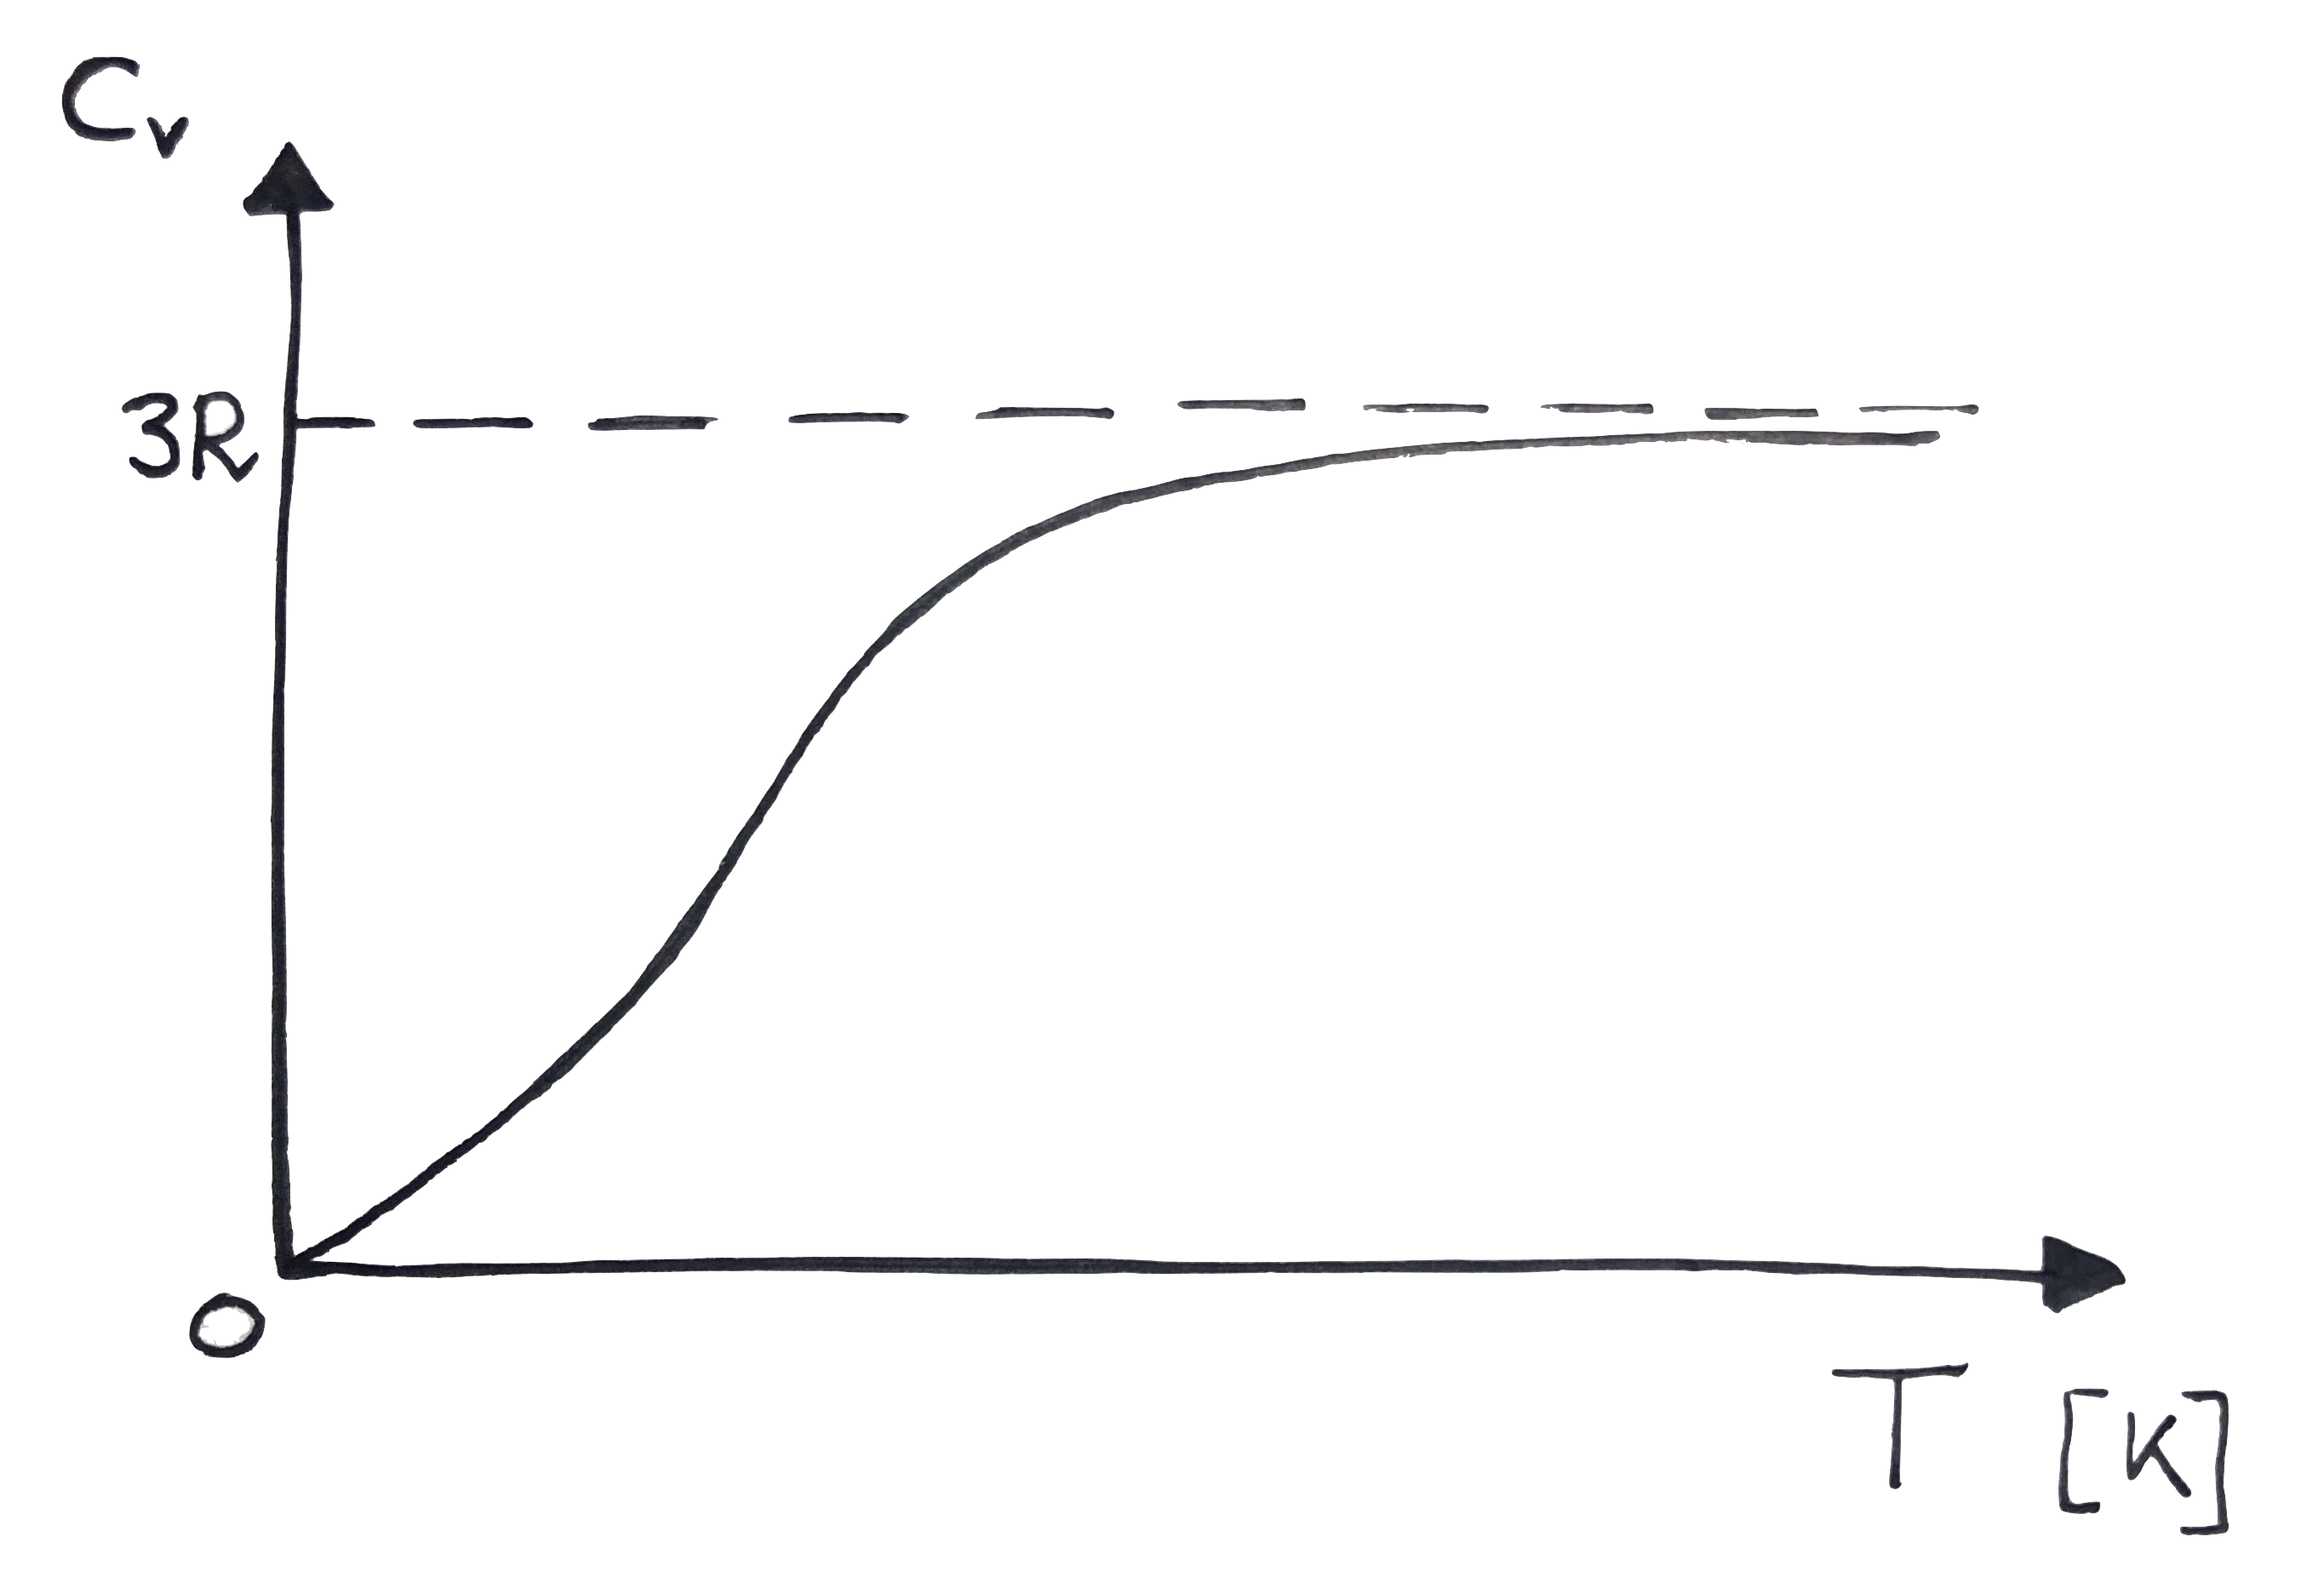
\includegraphics[scale=0.08]{/andamento_Cv}
\caption{andamento di $C_V$}
\end{figure}
Dove $R$ è la costante universale dei gas. 
Perciò si ha che $C_V = 3 R \simeq \SI{6}{cal / (mol * K)}$ che è la \underline{Legge di Dulong-Petit}, scoperta nel 1819, che afferma che i solidi hanno un calore specifico costante. 
Tuttavia sperimentalmente si osservò che tutto questo valeva solo a temperature elevate.
Nelle vicinanze dello zero assoluto invece il calore specifico tende a zero e a basse temperature ha un andamento del tipo $C_V \propto T^3$.

Fu Einstein a cercare di proporre un modello teorico che fosse più consistente con l'evidenza sperimentale nel 1905.
Egli ritenne che ad ogni mole di sostanza non si dovesse associare un'energia $kT$ bensì un termine che tenesse conto della quantizzazione.
Esattamente come fece Planck per il Corpo Nero, Einstein considerò che ogni mole di sostanza avesse un'energia data dal termine
$$E = \frac{ h \nu}{e^{ \frac{ h\nu}{k T } } - 1 }$$, 
pensando che il sistema non fosse altro che un insieme di $3 N_A$ oscillatori armonici semplici, aventi tutti la stessa frequenza di oscillazione.
Dunque per $n=1$:

\begin{equation}
\begin{cases}
	U = 3 N_A \frac{ h \nu}{e^{ \frac{ h \nu}{ k T} } - 1 } \\
	\beta = (k T)^{ -1 }
\end{cases}
\Rightarrow \quad C_V = \frac{ dU}{dT } = \frac{ 3 N_A}{k T^2 } (h \nu)^2 \frac{ e^{ \beta h \nu }}{\Bigl(  e^{ \beta h \nu } - 1   \Bigr)^2}
\end{equation}

Per temperature elevate, dunque per $\beta \sim 0$, si può esprimere l'esponenziale $e^{ \beta h \nu } = 1 + \beta h \nu + ...$
da cui $U(\beta \sim 0) = \frac{ 3 N_A h \nu}{\beta h \nu } = 3 N_A k T = 3 R T$ come avevano trovato Dulong e Petit.

Mentre nel caso di $k T \leq h \nu$ si nota che $C_V$ cala in quanto l'energia termica diventa confrontabile con la distanza fra i livelli energetici e dunque diventa rilevante la quantizzazione dell'energia.
In particolare per $k T \ll h \nu$ si ha che $\Bigl(  e^{ \beta h \nu } - 1  \Bigr) \sim e^{ \beta h \nu }$, perciò si ottiene, in accordo con l'evidenza sperimentale, che:

\begin{equation}
C_V = \frac{ 3 N_A (h \nu)^2}{k T^2 }e^{ - \beta h \nu } \quad \Rightarrow \quad \lim_{T \to 0} C_V = 0
\end{equation}

Dunque il modello di Einstein fu un notevole passo avanti, ma rimaneva ancora un problema: non si adattava, a basse energie, l'andamento come $T^3$ del calore specifico.
Ciò è da ricondurre ad un errore nelle assunzioni di Einstein: non c'era alcun motivo per cui le frequenze degli oscillatori armonici dovessero essere le stesse, anche perché questo avrebbe implicato l'esistenza di una frequenza caratteristica diversa per ogni materiale, ipotesi priva di fondamento.
A risolvere questi interrogativi fu Debye col suo modello nel 1912, che considerò come gli $N$ atomi avessero, in una mole di sostanza, un moto collettivo.
Il moto generale degli $N_A$ atomi è rappresentato dalla combinazione lineare di $3N_A$ modi di vibrazione ($N_A$ nel caso 1-D), ognuno avente una propria frequenza $\nu$.
A partire da questo sistema, Debye lo semplificò ulteriormente, pensando al solido come un sistema continuo.
Fece l'approssimazione di considerare onde longitudinali aventi il vincolo di avere nodi ai bordi del sistema.
Questo calcolo condusse ad un risultato quasi uguale a quello del Corpo Nero:

\begin{equation}
N(\nu)d\nu = \frac{ 4 \pi V}{v^3 } \nu^3 d\nu
\end{equation}

Dove si 4 al posto di 8 perché le onde elettromagnetiche sono anche trasversali e ovviamente si ha che $v \not = c$.
Tuttavia il sistema non è in verità continuo bensì discreto, per cui, per tenerne conto, Debye impose che:

\begin{equation}
\begin{split}
& \int_0^{\nu_m} N(\nu)d\nu = 3 N_A \quad \quad \mbox{dove $\nu_m$ è una \underline{frequenza di taglio}} \\
& \int_0^{\nu_m} \frac{ 4 \pi V}{v^3 } \nu^3 d\nu = 3 N_A \Rightarrow \frac{ 4 \pi V}{3 v^3 } \nu_m^3 = 3N_A \Rightarrow \nu_m = \Bigl(  \frac{ 3 N_A}{4 \pi V }  \Bigr)^{ \frac{ 1}{3 } }
\end{split}
\end{equation}

Ad ogni oscillatore viene associata una energia media $\varepsilon = \frac{ h \nu}{e^{ \frac{ h \nu}{k T } } - 1 }$, da cui si ottiene che:

\begin{equation}
\begin{split}
U & = \int_0^{\nu_m}  \frac{ h \nu}{e^{ \frac{ h \nu}{k T } } - 1 } \frac{ 4 \pi V}{v^3 } \nu^3  d\nu \quad \Rightarrow \quad
\begin{cases}
	\mbox{pongo:} \quad x \frac{ h \nu}{k T } \Rightarrow x_m = \frac{ h \nu_m}{k T } \\
	d\nu = \frac{ kT}{h } dx
\end{cases} \\
& = \frac{ 4 \pi V}{v^3 } \Bigl(  \frac{ kT}{h }  \Bigr)^4 h \int_0^{x_m} \frac{ x^3 dx}{e^x -1 } \\
& = \frac{ 9 R T}{x_m^3 } \int_0^{x_m} \frac{ x^3 dx}{e^x - 1 } \\
& = \frac{ 9 R T^4}{\Theta^3 } \int_0^{\Theta / T} \frac{ x^3 dx}{e^x -1 } \quad \mbox{con: } x_m = \frac{ \Theta}{T }
\end{split}
\end{equation}

Allora:
\begin{equation}
C_V = \frac{ dU}{dT } = 9R \Bigl[ 4 \Bigl(  \frac{ T}{\Theta }  \Bigr)^3 \int_0^{\Theta / T} \frac{ x^3 dx}{e^x -1 } - \frac{ \Theta}{T }\frac{ 1}{e^{ \frac{ \Theta}{T } } - 1 } \Bigr]
\end{equation}

Dunque:
\begin{equation}
\Theta = \frac{ h}{k } \Bigl(  \frac{ 9N_A}{4 \pi V }  \Bigr)^{ \frac{ 1}{3 } } v
\end{equation}
è una temperatura oltre la quale tutti i modi di vibrazione sono attivi.

Vediamo la $\Theta$ di alcuni materiali:
\begin{table}[h]
\centering
\begin{tabular}{|l|l|}
\hline
\textbf{Sostanza}    & \textbf{$\Theta$} \\ \hline
Elio solido & 30 K     \\ \hline
Ferro       & 465 K    \\ \hline
Diamante    & 1860 K   \\ \hline
\end{tabular}
\end{table}


\begin{equation}
\begin{split}
& \mbox{Se} \quad T \ll \Theta \Rightarrow \frac{ \Theta}{T } \sim \infty \Rightarrow 9R \frac{ T^4}{\Theta^3} \int_0^{\infty} \frac{ x^3 dx}{e^x - 1} = \frac{ 3}{5 } \pi^4 R \Bigl(  \frac{ T^4}{ \Theta^3}  \Bigr) \\
& \Rightarrow C_V = \frac{ 12}{5 } \pi^4 R \Bigl(  \frac{ T}{\Theta }  \Bigr)^3 \quad \mbox{ed ecco l'attesa dipendenza da $T^3$} \\
& \mbox{Se} \quad T \gg \Theta \mbox{, si ha che} \quad e^x = 1 + x + ... \quad (x \sim 0) \\
& \Rightarrow U = \frac{ 9R T^4}{\Theta^3 } \int_0^{\frac{ \Theta}{ T}} \frac{ x^3}{x }dx = \frac{ 9 R T^4}{3 \Theta^3 } \frac{ \Theta^3}{T^3 } = 3RT \quad \mbox{Come scoperto da Dulong-Petit}
\end{split}
\end{equation}
Il modello di Debye è semplice ma grazie alle sue assunzioni fornisce, per usando la statistica di Maxwell-Boltzmann, risultati eccellenti.
È lecito usare la statistica classica in quanto i modi sono distinguibili nel reticolo cristallino.
Occorre fare delle considerazioni sui contributi a $C_V$:

\begin{equation}
\begin{cases}
	\mbox{Contributo reticolare} \quad C_V = \frac{ 12}{5 } \pi^4 R \Bigl(  \frac{ T}{\Theta }  \Bigr)^3 \\
	\mbox{Contributo elettronico} \quad C_V = \frac{ \pi^2}{2 } N k \Bigl(  \frac{ T}{T_F}  \Bigr) \\
\end{cases}
\Rightarrow \frac{ C_{VR}}{C_{VE} } = \frac{ 5}{24 \pi^2 }\frac{ N}{N_A } \frac{ \Theta^3}{T^2 T_F } \Rightarrow T_0 \simeq \Bigl(  \frac{ \Theta}{T_F }  \Bigr)^{ \frac{ 1}{2 } } \Theta
\end{equation}
Oltre la temperatura $T_0$ il contributo reticolare è maggiore di quello elettronico.
Quello elettronico supera quello reticolare solo quando si è vicini allo zero assoluto per i metalli, dove ci si aspetta quindi un andamento lineare. 


























